\documentclass{report}

%subject to pathing issues, remember to change
\input{../../pkgs/preamble}
\input{../../pkgs/macros}
\input{../../pkgs/letterfonts}


\title{\Huge{Calc4}\\ Notes }
\author{\huge{Yan Bogdanovskyy (yawnbo)}}
\date{\today}

\begin{document}
\begin{center}
% making blank spaces between the below makes the compiler VERY unhappy so i'm leaving it as a mess
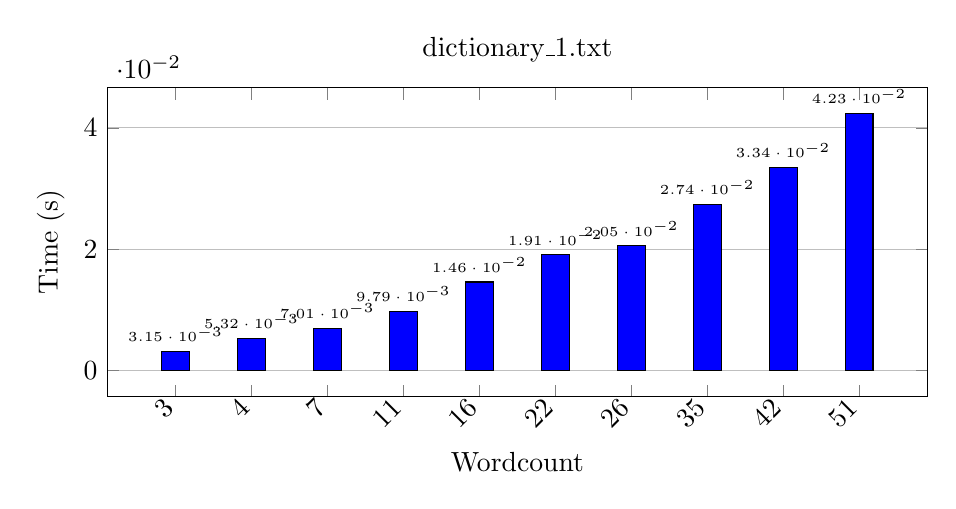
\begin{tikzpicture}
\begin{axis}[
    title={dictionary\_1.txt},
    xlabel={Wordcount},
    ylabel={Time (s)},
    ymajorgrids=true,
    xtick=data,
    ymin=0,
    bar width=10pt,
    width=12cm,
    height=5.5cm, % this and the above one can be changed to look nicer but i just do this to keep at one page
    enlargelimits=0.1,
    symbolic x coords={3,4,7,11,16,22,26,35,42,51},
    xticklabel style={rotate=45, anchor=east},
    nodes near coords,
    every node near coord/.append style={font=\tiny},
]
% actual data goes here, this is just piped from the times.txt file.
\addplot[ybar,fill=blue] coordinates {
    (3,0.0031483) (4,0.0053236) (7,0.00701221) (11,0.0097928)
    (16,0.0146107) (22,0.0190672) (26,0.0205466) (35,0.0273532)
    (42,0.0334335) (51,0.0423388)
};
\end{axis}
\end{tikzpicture}

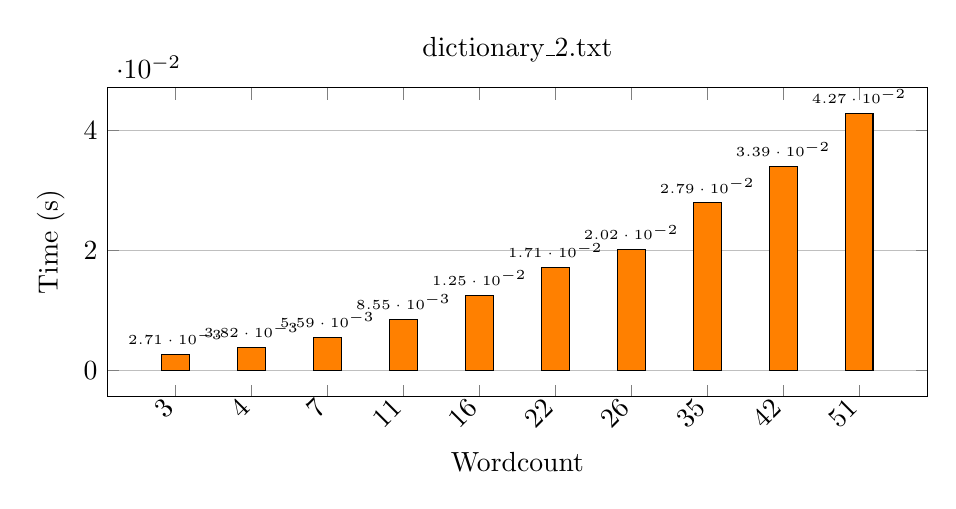
\begin{tikzpicture}
\begin{axis}[
    title={dictionary\_2.txt},
    xlabel={Wordcount},
    ylabel={Time (s)},
    ymajorgrids=true,
    xtick=data,
    ymin=0,
    bar width=10pt,
    width=12cm,
    height=5.5cm,
    enlargelimits=0.1,
    symbolic x coords={3,4,7,11,16,22,26,35,42,51},
    xticklabel style={rotate=45, anchor=east},
    nodes near coords,
    every node near coord/.append style={font=\tiny},
]
\addplot[ybar,fill=orange] coordinates {
    (3,0.0027129) (4,0.0038152) (7,0.0055854) (11,0.00854661)
    (16,0.0125299) (22,0.0171363) (26,0.0201639) (35,0.0279095)
    (42,0.0339298) (51,0.042746)
};
\end{axis}
\end{tikzpicture}

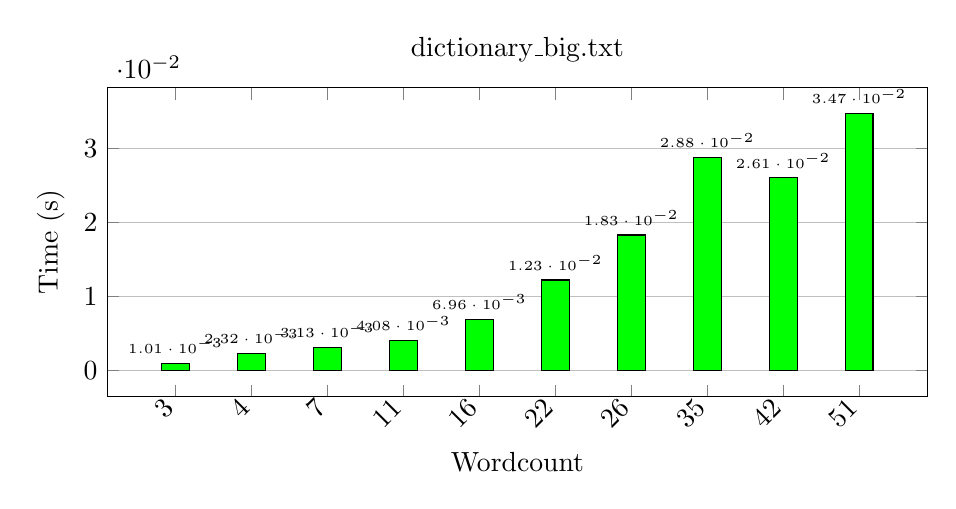
\begin{tikzpicture}
\begin{axis}[
    title={dictionary\_big.txt},
    xlabel={Wordcount},
    ylabel={Time (s)},
    ymajorgrids=true,
    xtick=data,
    ymin=0,
    bar width=10pt,
    width=12cm,
    height=5.5cm,
    enlargelimits=0.1,
    symbolic x coords={3,4,7,11,16,22,26,35,42,51},
    xticklabel style={rotate=45, anchor=east},
    nodes near coords,
    every node near coord/.append style={font=\tiny},
]
\addplot[ybar,fill=green] coordinates {
    (3,0.001011) (4,0.0023207) (7,0.0031338) (11,0.0040783)
    (16,0.0069565) (22,0.0122559) (26,0.0183288) (35,0.0288018)
    (42,0.0260532) (51,0.0347362)
};
\end{axis}
\end{tikzpicture}

% don't know how this one performed better but i assume it has to do with the fact that this doesn't count alloc time for the table?
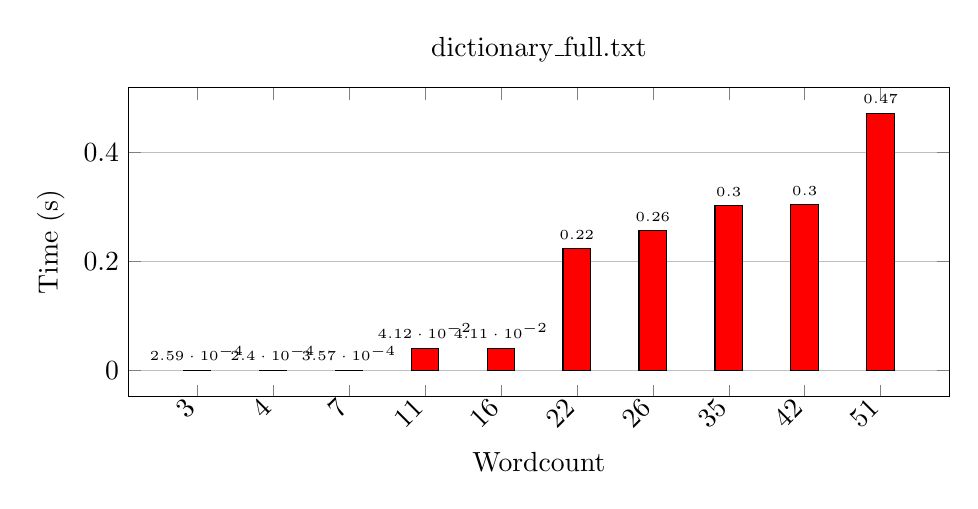
\begin{tikzpicture}
\begin{axis}[
    title={dictionary\_full.txt},
    xlabel={Wordcount},
    ylabel={Time (s)},
    ymajorgrids=true,
    xtick=data,
    ymin=0,
    bar width=10pt,
    width=12cm,
    height=5.5cm,
    enlargelimits=0.1,
    symbolic x coords={3,4,7,11,16,22,26,35,42,51},
    xticklabel style={rotate=45, anchor=east},
    nodes near coords,
    every node near coord/.append style={font=\tiny},
]
\addplot[ybar,fill=red] coordinates {
    (3,0.0002593) (4,0.00024) (7,0.0003567) (11,0.0411706)
    (16,0.0411257) (22,0.223422) (26,0.256378) (35,0.301979)
    (42,0.303743) (51,0.471139)
};
\end{axis}
\end{tikzpicture}
\end{center}
% i'm free!!!!!!!!!!!!!!!!!!!!!!!!!!!!!!!!!!!!!!!!!!!
\end{document}
